\documentclass[12pt, letterpaper]{article}
\usepackage{amsmath,amssymb}
\usepackage{graphicx,float}

\begin{document}
\title{Reverse Kinematics on a General Four-Bar Linkage using a Least Squares Curve Fit Algorithm--A Work In Progress}
\author{Joshua Holbrook}
\date{November 19th 2008}
\maketitle

\section*{The Standard Kinematics Problem}
\subsection*{Adopted Conventions}
For a general four-bar linkage:

\begin{figure}[H]
\caption A Model for a Four-Bar Linkage
\centering
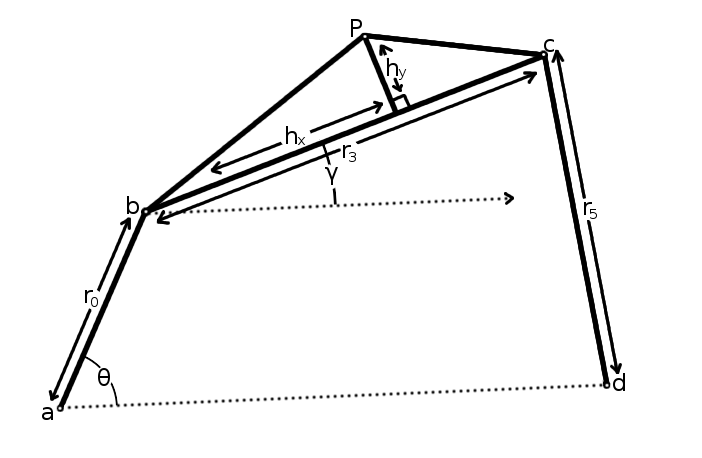
\includegraphics[width=4in]{fourbar}
\label{fig:fourbar}
\end{figure}

\(a\), \(b\), \(c\), \(d\) and \(p\) are vectors in \(\mathbb{R}^2\), and \(x\) is a vector using basis vectors \(\left(c-b\right)\) and \(R_{\frac{\pi}2}\left(c-b\right)\) where \(R_{\frac{\pi}2}\) is a 90 degree counter-clockwise rotation matrix. \(r_1\), \(r_3\) and \(r_5\) are fairly standard notation (from what I've seen) for the lengths of the input, transmission and output links, respectively. \(r_2\), \(r_4\) and \(r_6\) are unlabeled in this diagram because I don't expect that I'll need them (\(r_2\) and \(r_4\) could have been used to calculate \(p\) instead of \(h\), but \(h\) should be more convenient for the purposes of solving this problem). \(\theta\) and \(\gamma\) are the input and transmission angles, respectively.

To clarify: For my purposes, the rotation matrix \(R_{\theta}\), which is used extensively in these equations, is defined as:

\[R_{\theta}=\begin{bmatrix}\cos \theta & \sin \theta \\ -\sin \theta & \cos \theta \end{bmatrix}\]

\(a, d, r_1, r_3, r_5, h\) and \(\theta\) are given for this problem, and the goal is to calculate the position \(p\).

Calculating \(b\) is easy:

\[b=a+r_1\begin{pmatrix}\cos\theta \\ \sin\theta\end{pmatrix}\]

The next part, however, gets more difficult.

Perhaps the most straightforward approach conceptually is simply to solve the sytem of equations:

\begin{align*}||c-b||^2=r_3^2\\
||c-d||^2=r_5^2\end{align*}

or, in other words,
\begin{align*}(c-b)^T(c-b)=r_3^2\\
(c-d)^T(c-d)=r_5^2\end{align*}

The problem with this approach, of course, is that there are \emph{two} solutions to this system of equations, as illustrated in figure \ref{fig:dyad}:

\begin{figure}[H]
\caption{There are \emph{Two} Solutions.} 
\label{fig:dyad}
\centering
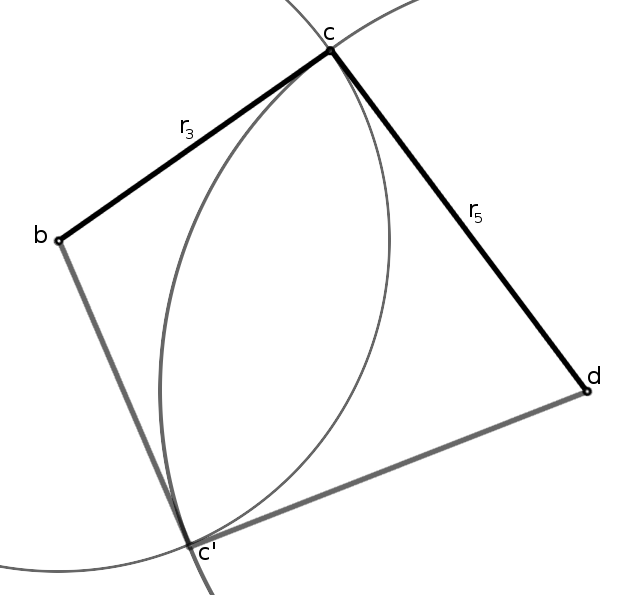
\includegraphics[width=3in]{dyad}
\end{figure}

This sort of linkage, where there is more than one valid position for it to be in given lengths and end positions, is (from what I can tell) called a dyad.

If this problem were being solved on paper (with the graphics method, even), this part would be a minor hurdle--simply find the two solutions and pick the one that makes sense in context. However, this simply won't do for my purposes.

One approach I considered was to isolate one by adding this third restriction:

\[(c-b)^T\left(R_{\frac{\pi}2}(d-b)\right) \ge 0\]

This equation creates a vector orthogonal to \((d-b)\) by using a \(90^o\) rotation and requires that the dot product of this vector with \((c-b)\) be less than zero; In other words, the angle formed between these two vectors must be less than \(90^o\).

However, this system of equations, as far as I know, doesn't have an analytical solution, meaning that my final equation won't be analytically differentiable (more on that later). I can get around this pretty easily through numerical techniques, but I'd at least like to explore analytical alternatives.

An alternative approach I have is to use the law of cosines to find the (cosine of the) angle between \((c-b)\) and \((d-b)\), here denoted as \(\phi\):

\[\cos\phi = \frac{r_3^2+||d-b||^2-r_5^2}{2r_3||d-b||}\]

then find \((c-b)\) by re-scaling and rotating \((d-b)\):

\[(c-b)_{upper}=\begin{pmatrix}\cos\phi & \sqrt{1-\left(\cos\phi\right)^2}\\
-\sqrt{1-\left(\cos\phi\right)^2} & \cos\phi\end{pmatrix}\frac{r_3}{||d-b||}(d-b)\]

%Figure out the second solution

\[(c-b)_{lower}=\begin{pmatrix}\cos\phi & -\sqrt{1-\left(\cos\phi\right)^2}\\
\sqrt{1-\left(\cos\phi\right)^2} & \cos\phi\end{pmatrix}\frac{r_3}{||d-b||}(d-b)\]

This should take care of the double-solution and the non-analytical problems, but it also ends up being quite complex when everything is written out in full, with the equations for \(\cos\phi\) and \(b\) substituted into this equation. Also worth thinking about is that the euclidean norms in this equation aren't particularly easy to compute either. This complexity is something that may work against this method, especially if I analytically differentiate this monster by hand. Still, it can be done.

Finally is the business of finding p. As previously stated, I can do use the lengths \(r_2\) and \(r_4\) along with points \(b\) and \(c\) (now found) to find \(p\). However, since the lengths and positions of everything in this problem are static, it will be easier to simply specify the position of \(p\) along a basis made up of vectors \((c-b)\) and \(R_{\frac{\pi}2}(c-b)\):

\[p=\begin{pmatrix}\uparrow & \uparrow \\
\left(c-b\right) & R_{\frac{\pi}2}\left(c-b\right)\\
\downarrow & \downarrow\end{pmatrix}h + b\]

Put all these together, and a single analytical equation \(p(r_1,r_3,r_5,a,d,h,\theta)\) results. It's nasty, but solving it is relatively straightforward.

Another paramater that may be interesting to know is the transmission angle, \(\gamma\). Luckily, this one is easy to figure out with an application of the geometric interpretation of the dot product between \((c-b)\) and \((d-a)\):

\[\gamma=\cos^{-1}\left(-\frac{(c-b)^T(d-a)}{||d-a||r_3}  \right)\]

Finally, there are many cases where there is no solution to this problem--specifically, I'm referring to the cases where the input angle has limits. Specifically, there are (to my knowledge) four cases I'll have to worry about. From a lab report I wrote some time ago ("Taxonomic Schemes of the Four-Bar Linkage"):

\begin{flalign*}
  \textbf{Case 1:} & r_1+r_6 \leq r_3+r_5, |r_1-r_6| \geq |r_3-r_5| \\ 
  \textbf{Case 2:} & r_1+r_6 > r_3+r_5, |r_1-r_6| > |r_3-r_5| \\
  \textbf{Case 3:} & r_1+r_6 < r_3+r_5, |r_1-r_6| < |r_3-r_5| \\
  \textbf{Case 4:} & r_1+r_6 > r_3+r_5, |r_1-r_6| < |r_3-r_5|
\end{flalign*}

where, in this case \(r_6=||d-a||\).

From the same lab report comes figure \ref{fig:limits}, revised for this document:

\begin{figure}[H]
\centering
\caption{Hand-Drawn Diagrams Detailing Linkage Positions at Maximum and Minimum Input Angles.}
\label{fig:limits}
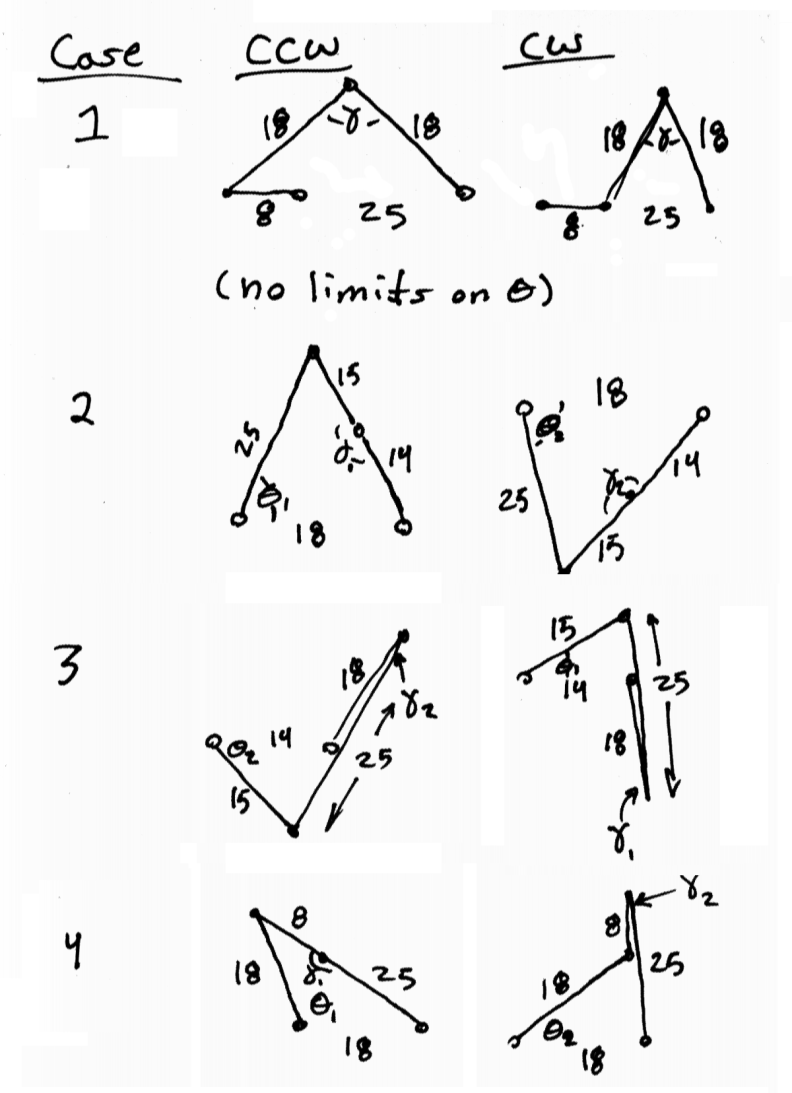
\includegraphics[width=4.0in]{position_diagrams}
\end{figure}

These were for specific dimensions, but the relationships should still hold. The first case is ideal, in that there are no limits to \(\theta\). Finding the inner and outer limit positions for the others consists of solving for \(\theta\) in

\[\cos\theta=\frac{r_1^2+r_6^2-c^2}{2r_1r_6}\]

Where c is as follows:

\begin{table}[H]
  \centering
  \caption{Parameter c For The Purposes of Calculating Limit Angles}
  \begin{tabular}{r*{2}{l}} 
    Cases & Outer & Inner \\\hline
    2 & \(r_3+r_5\) & \(r_3+r_5\)\\
    3 & \(r_3-r_5\) & \(r_3-r_5\)\\
    4 & \(r_3+r_5\) & \(r_5-r_3\)
  \end{tabular}
  \label{tab:limit_param}
\end{table}

This means that \(\theta\) is limited in the following cases to:

\begin{table}[H]
  \centering
  \caption{Limit Positions}
  \begin{tabular}{r l} 
    Cases & Limits for Theta  \\ \hline
    1 & \(\left[\pi,-\pi\right]\)\\ \;
    2 & \(\left[ -\cos^{-1}\frac{r_1^2+r_6^2-(r_3+r_5)^2}{2r_1r_6}, \cos^{-1}\frac{r_1^2+r_6^2-(r_3+r_5)^2}{2r_1r_6}\right]\) \\ \;
    3 & \(\left[ \cos^{-1} \frac{r_1^2+r_6^2-(r_3-r_5)^2}{2r_1r_6},2\pi-\frac{r_1^2+r_6^2-(r_3-r_5)^2}{2r_1r_6} \right]\) \\ \;
    4 & \(\left[ \cos^{-1}\frac{r_1^2+r_6^2-(r_5+r_3)^2}{2r_1r_6},\frac{r_1^2+r_6^2-(r_5+r_3)^2}{2r_1r_6} \right] \)
  \end{tabular}
  \label{tab:limit_posish}
\end{table}

\section*{The Reverse Kinematics Problem}
\subsection*{Difficulties}
Being able to calculate the position of p for a given set of parameters is worth being able to do, but in design, the inverse is what's desirable to calculate in most cases; That is, one usually wants to design a four-bar linkage such that it can reach a certain set of positions with certain transmission angles.

This problem, being completely non-linear, is very difficult to solve. It's made even worse by the fact that there may be multiple solutions with varying numbers of free variables, or possibly no solutions at all.

There are a number of approaches to this problem.  The oldest method is trial and error--come up with some numbers, use the graphics method to plot the path, and adjust the linkage in some intelligent ways and repeat until the path is found.

Another general method for solving linkage problems involves solving a series of polynomial equations (such as \(u^Tu=||u||\) where \(c\) and \(s\) are substituted for \(\cos\theta\) and \(\sin\theta\) respectively and are constrained such that \(s^2 + c^2 = 1\)) and using a Gaussian Elimination-like algorithm to arrive at a solution (that I don't know much about). There are other high-level advanced methods for solving such equations, both analytical (in this simple case) and numerically. However, I instead plan to solve this problem using principles from optimization.

\subsection*{An Optimization Approach}

I should be able to find solutions to this problem by solving the following optimization problem:

\[\min \sum_{i=1}^n\bigg|\bigg|\begin{pmatrix}\bar{p} \\ \bar{\gamma}\end{pmatrix}_i -
\begin{pmatrix}p(r_1,r_3,r_5,a,d,h,\theta_i) \\ \gamma(r_1,r_3,r_5,a,d,h,\theta_i)\end{pmatrix} \bigg|\bigg|^2\]

where \(r_1,r_3,r_5,a,d,h\) and all the \(\theta_i\) are free, and \(\bar{p}_i\) and \(\bar{\gamma}_i\) are points one wants the curve to go through. This ends up being a sort of least squares curve fitting problem, and can be solved using the Gauss-Newton method assuming the constraints on \(\theta\) never come into play.

One advantage of using a curve fit over other methods is that, even if there isn't a possible exact solution, the problem should still converge on a minimum that is, by a measure (likely a familiar measure), the closest path to all the points.

\section*{Currently Unresolved Issues}
\subsection*{Will This Really Work?}
Even for a relatively simple application of curve fitting, this seems very complex to me, and I wouldn't be surprised if I missed a way in which this could "break."
\subsection*{Dealing with constraints}
Unconstrained optimization is fairly easy. Constrained optimization is a much harder problem, especially when the equations involved become non-linear. I \emph{do} have constraints to deal with, and as of yet I'm not sure how. My current idea is to modify \(p\) such that it has a solution for \(\theta\) outside the domain of the function, plus a penalty function to make the objective function extra-large for \(\theta\) outside the domain.  For example, I may use the function

\begin{align*}\tilde{p}(\theta)=&p(\theta) \text{ for } \theta \in [\theta_1,\theta_2]\\
&p(\theta_{1})+\frac{dp}{d\theta}\bigg|_{\theta_1}\theta+(\theta_1-\theta)^{12} \text{ for } \theta < \theta_1\\
&p(\theta_{2})+\frac{dp}{d\theta}\bigg|_{\theta_2}\theta+(\theta-\theta_2)^{12} \text{ for } \theta > \theta_2\end{align*}

The penalty is pretty arbitrary at this point.



\end{document}

